\documentclass[tikz,border=12pt]{standalone}
\usepackage{amsmath}
\usepackage{tikz}
\usetikzlibrary{3d,shapes.geometric,arrows.meta,calc}

\begin{document}
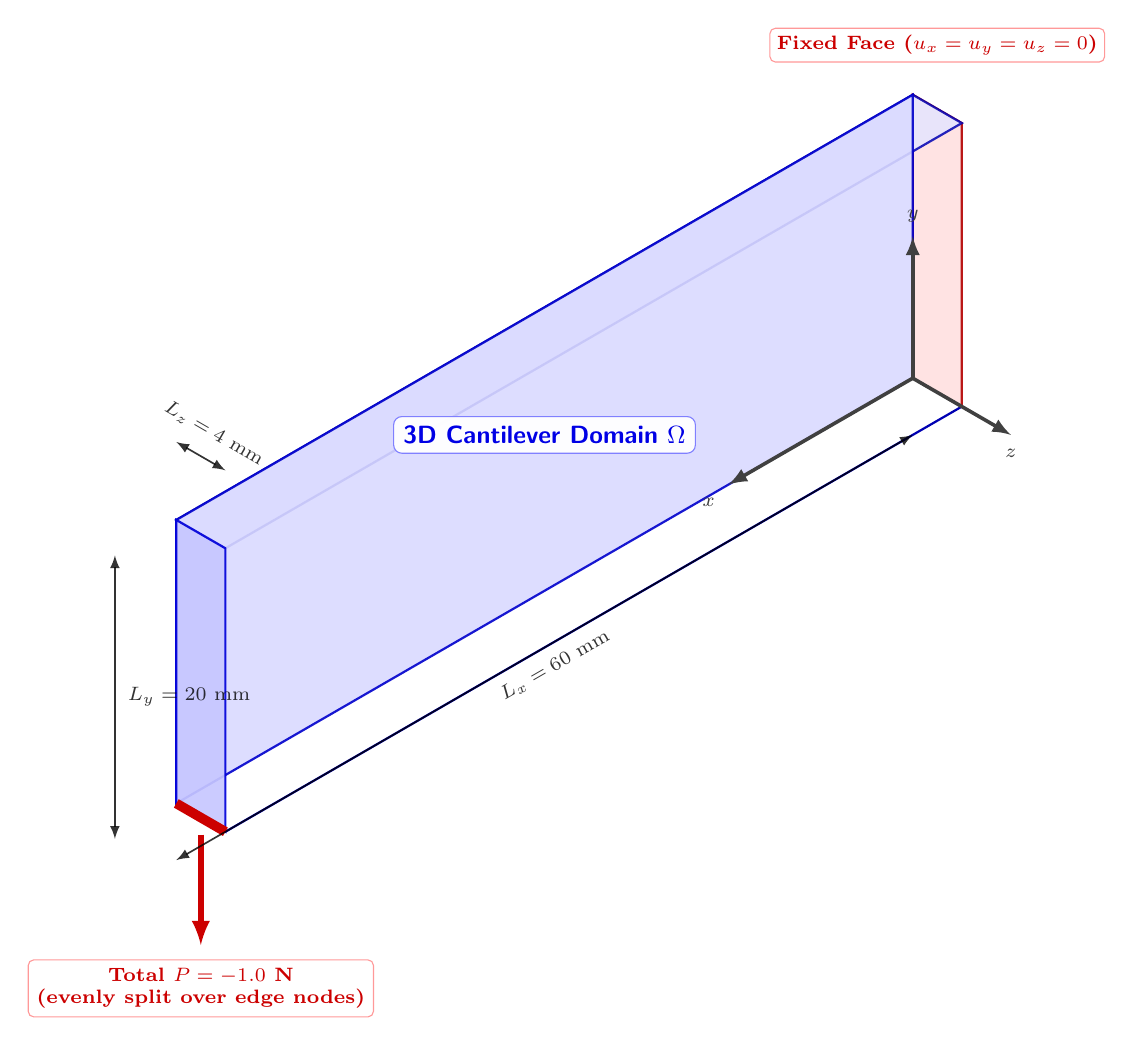
\begin{tikzpicture}[x={(-0.866cm,-0.5cm)}, y={(0.866cm,-0.5cm)}, z={(0cm,1cm)}, scale=1.8, >=latex]
  % ============================================================
  % 坐标映射 (与 CantileverRightBottomEdge3d 代码坐标系精确一致):
  %   TikZ x = 代码 x = 长度 Lx
  %   TikZ y = 代码 z = 宽度 (屏幕右下方向)
  %   TikZ z = 代码 y = 高度 (屏幕竖直方向)
  % ============================================================
  \def\Lx{6.0}   % 长度 60 mm
  \def\Ly{0.4}   % 宽度 (代码 z) 4 mm
  \def\Lz{2.0}   % 高度 (代码 y) 20 mm

  % 1. Box faces (back-to-front)
  % 左端固支面 (代码 x=0)
  \draw[thick, fill=red!12, draw=red!70!black, opacity=0.9]
    (0,0,0) -- (0,\Ly,0) -- (0,\Ly,\Lz) -- (0,0,\Lz) -- cycle;
  % 顶面 (代码 y=L_y)
  \draw[thick, fill=blue!10, draw=blue!70!black, opacity=0.85]
    (0,0,\Lz) -- (\Lx,0,\Lz) -- (\Lx,\Ly,\Lz) -- (0,\Ly,\Lz) -- cycle;
  % 前面 (代码 z=0)
  \draw[thick, fill=blue!15, draw=blue!80!black, opacity=0.9]
    (0,0,0) -- (\Lx,0,0) -- (\Lx,0,\Lz) -- (0,0,\Lz) -- cycle;
  % 右端面 (代码 x=L_x)
  \draw[thick, fill=blue!22, draw=blue!85!black, opacity=0.92]
    (\Lx,0,0) -- (\Lx,\Ly,0) -- (\Lx,\Ly,\Lz) -- (\Lx,0,\Lz) -- cycle;
  % 底面后缘棱线
  \draw[thick, draw=blue!70!black] (0,\Ly,0) -- (\Lx,\Ly,0);

  % 2. Domain label
  \node[font=\small\bfseries\sffamily, color=blue!90!black,
        fill=white, fill opacity=0.95, text opacity=1.0, inner sep=3.5pt, rounded corners=3pt, draw=blue!50]
        at (\Lx*0.5, 0, \Lz*0.55) {3D Cantilever Domain $\Omega$};

  % 3. Fixed left end face (u = 0)
  \node[red!80!black, font=\scriptsize\bfseries, align=center,
        fill=white, fill opacity=0.95, text opacity=1.0, inner sep=2.5pt, rounded corners=2pt, draw=red!40]
        at (0, \Ly*0.5, \Lz+0.45) {Fixed Face ($u_x=u_y=u_z=0$)};

  % 4. Loaded right bottom edge (代码 x=Lx, y=0, 沿 z 宽度), 总力沿 -y (屏幕竖直向下)
  \draw[line width=3.5pt, red!80!black] (\Lx,0,0) -- (\Lx,\Ly,0);
  \draw[->, ultra thick, red!80!black, line width=2.0pt]
    (\Lx, \Ly*0.5, -0.12) -- (\Lx, \Ly*0.5, -0.9);
  \node[below, red!80!black, font=\scriptsize\bfseries, align=center,
        fill=white, fill opacity=0.95, text opacity=1.0, inner sep=3pt, rounded corners=2pt, draw=red!40]
        at (\Lx, \Ly*0.5, -1.0) {Total $P = -1.0\text{ N}$\\(evenly split over edge nodes)};

  % 5. 坐标轴 (原点: 左前下角, 与代码坐标系一致: x=长度, y=高度, z=宽度)
  \draw[->, line width=1.3pt, black!75] (0,0,0) -- (1.5,0,0)
    node[below left=1pt, black!75, font=\scriptsize\bfseries] {$x$};
  \draw[->, line width=1.3pt, black!75] (0,0,0) -- (0,0,1.0)
    node[above=1pt, black!75, font=\scriptsize\bfseries] {$y$};
  \draw[->, line width=1.3pt, black!75] (0,0,0) -- (0,0.8,0)
    node[below=1pt, black!75, font=\scriptsize\bfseries] {$z$};

  % 6. Dimensions
  % 长度 Lx (底面下方)
  \draw[<->, opacity=0.8, semithick] (0,0,-0.4) -- (\Lx,0,-0.4)
    node[midway, sloped, below=1pt, font=\scriptsize] {$L_x = 60\text{ mm}$};
  % 高度 L_y (右端面右侧竖直, 代码 y = 高度)
  \draw[<->, opacity=0.8, semithick] (\Lx+0.5,0,0) -- (\Lx+0.5,0,\Lz)
    node[midway, right=1pt, font=\scriptsize] {$L_y = 20\text{ mm}$};
  % 宽度 L_z (右端顶面上方沿宽度方向, 代码 z = 宽度)
  \draw[<->, opacity=0.8, semithick] (\Lx,0,\Lz+0.55) -- (\Lx,\Ly,\Lz+0.55)
    node[midway, sloped, above=3pt, font=\scriptsize] {$L_z = 4\text{ mm}$};
\end{tikzpicture}
\end{document}
